% WAAM Digital Twin — Formula Reference (illustrated, newbie-friendly)
% Compile: pdflatex WAAM_FORMULAE.tex   (run twice for TOC / refs)
% Needs: amsmath, tikz (standard TeX Live)
\documentclass[11pt,a4paper]{article}

\usepackage[margin=22mm]{geometry}
\usepackage{amsmath,amssymb,bm}
\usepackage{booktabs}
\usepackage{enumitem}
\usepackage{xcolor}
\usepackage{hyperref}
\usepackage{tikz}
\usetikzlibrary{arrows.meta,calc,decorations.pathmorphing,fit,positioning,shapes.geometric,patterns}

\hypersetup{colorlinks=true,linkcolor=blue!50!black,citecolor=blue!40!black,urlcolor=blue!60!black}

\title{WAAM Digital Twin --- Formula Reference\\
\large Illustrated guide aligned with \texttt{waam\_twin}}
\author{waam\_twin project}
\date{\today}

\newcommand{\dd}{\mathrm{d}}
\newcommand{\vect}[1]{\mathbf{#1}}
\newcommand{\unit}[1]{\hat{\vect{#1}}}
\newcommand{\fref}[1]{\par\smallskip\noindent\textit{References:} #1\par}
\newcommand{\code}[1]{\texttt{\detokenize{#1}}}
\newcommand{\newbie}[1]{\par\medskip\noindent\textit{In plain words:} #1\par\medskip}
\newcommand{\incode}[1]{\par\smallskip\noindent\textit{In the code:} #1\par}
% Allow long paths / code tokens to break at punctuation
\usepackage{xurl}

\begin{document}
\maketitle

\begin{abstract}
This document explains every major equation used by the WAAM (Wire Arc Additive
Manufacturing) digital twin --- not only the symbols, but \emph{what they mean},
\emph{why they appear}, and \emph{how the current \texttt{waam\_twin} code uses them}.

The twin is a GPU continuum melt-pool simulator (Taichi): lattice Boltzmann flow
(D3Q19), enthalpy--porosity phase change, VOF free surface, and a catalogue of
weld-pool forces. Equations below are grouped by physics domain and matched to
\texttt{solvers/coupled\_step.py}, \texttt{kernels/}, and \texttt{physics/}
as of the current repository (Gaussian / Goldak heat sources, Lin--Eagar arc
pressure, energy-normalized injection, physics tiers \texttt{thermal}/\texttt{flow}/\texttt{full}).
\end{abstract}

\tableofcontents
\newpage

%=============================================================================
\section{How to read this document}
%=============================================================================

Think of the twin as answering: \emph{``Given current, voltage, wire feed, and
torch motion, what does the melt pool and bead look like?''}

\begin{center}
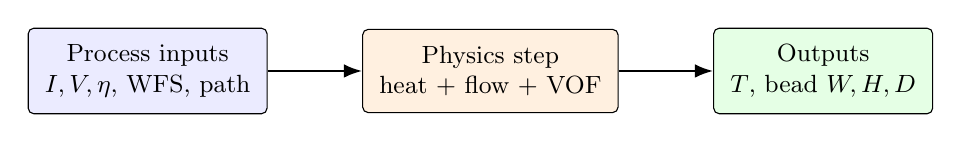
\begin{tikzpicture}[
  box/.style={draw,rounded corners=2pt,align=center,inner sep=6pt,font=\small},
  arr/.style={-{Latex},thick}
]
\node[box,fill=blue!8] (in) {Process inputs\\$I,V,\eta$, WFS, path};
\node[box,fill=orange!12,right=12mm of in] (phys) {Physics step\\heat + flow + VOF};
\node[box,fill=green!10,right=12mm of phys] (out) {Outputs\\$T$, bead $W,H,D$};
\draw[arr] (in) -- (phys);
\draw[arr] (phys) -- (out);
\end{tikzpicture}
\end{center}

\begin{itemize}[leftmargin=*]
  \item Each subsection starts with a short \textbf{plain-words} explanation.
  \item Then the equation(s), then a short note on \textbf{where the code does it}.
  \item TikZ sketches show geometry / energy flow; they are conceptual, not CAD.
\end{itemize}

\textbf{Notation habit.} Capital $Q$ is usually a \emph{power} [W].
Lower-case $q$ is usually a \emph{flux or density} [W/m$^2$ or W/m$^3$], or
line energy [J/m]. Subscripts: $\mathrm{eff}$ = after efficiency,
$\mathrm{arc}$ = arc source field.

%=============================================================================
\section{Process inputs and energy balance}
%=============================================================================

\subsection{Electrical arc power and effective heat}
\label{sec:qeff}

\newbie{The welding power supply pushes current $I$ through an arc with voltage
$V$. Their product $IV$ is the electrical power. Only a fraction $\eta$ of that
power actually heats the workpiece --- the rest is lost to radiation, the arc
column, spatter, etc. That useful part is $Q_{\mathrm{eff}}$.}

\begin{align}
  P &= IV \label{eq:arc-power}\\
  Q_{\mathrm{eff}} &= \eta\, IV \label{eq:qeff}
\end{align}

\begin{center}
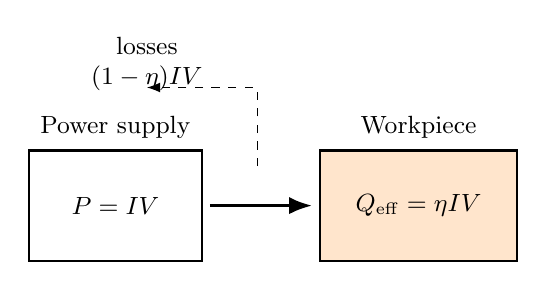
\begin{tikzpicture}[font=\small]
  \draw[thick] (0,0) rectangle (2.2,1.4);
  \node at (1.1,1.7) {Power supply};
  \node at (1.1,0.7) {$P=IV$};
  \draw[-{Latex},very thick] (2.3,0.7) -- (3.6,0.7);
  \draw[thick,fill=orange!20] (3.7,0) rectangle (6.2,1.4);
  \node at (4.95,1.7) {Workpiece};
  \node at (4.95,0.7) {$Q_{\mathrm{eff}}=\eta IV$};
  \draw[-{Latex},dashed] (2.9,1.2) -- (2.9,2.2) -- (1.5,2.2);
  \node[align=center] at (1.5,2.5) {losses\\$(1-\eta)IV$};
\end{tikzpicture}
\end{center}

Typical GMAW steel: $\eta \sim 0.6$--$0.85$. Your example jobs often use
$\eta \approx 0.72$ (\code{process.arc_efficiency}).

\incode{\code{twin.Q_w} stores electrical power $IV$\,[W].
Efficiency \code{twin.eta} is applied in the heat kernels so exactly
$\eta Q_w\Delta t$ joules enter metal each step
(\path{kernels/thermal.py}: \code{inject_arc_heat}, \code{inject_goldak_heat}).
Do \emph{not} bake $\eta$ into \code{Q_w} twice.}

\fref{\cite{Kou2003,Incropera2007,Radaj2003}}

\subsection{How $Q_{\mathrm{eff}}$ relates to $\dot{q}_{\mathrm{arc}}$}
\label{sec:qarc-vs-qeff}

\newbie{$Q_{\mathrm{eff}}$ is one number: ``how many watts of useful heat?''
$\dot{q}_{\mathrm{arc}}(x,y,z)$ is a 3D map: ``how many watts per cubic metre
at each point?'' The map is shaped by Gaussian or Goldak. If you integrate the
map over the whole domain you must recover $Q_{\mathrm{eff}}$.}

\begin{equation}
  \int_{\Omega} \dot{q}_{\mathrm{arc}}(\vect{x})\,\dd V
  \;=\; Q_{\mathrm{eff}} \;=\; \eta\, IV
  \label{eq:qarc-integral}
\end{equation}

\begin{center}
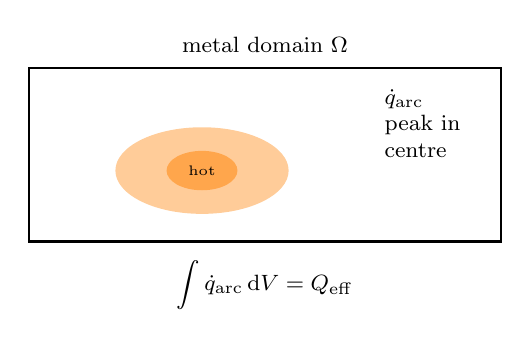
\begin{tikzpicture}[font=\footnotesize]
  \draw[thick] (0,0) -- (6,0) -- (6,2.2) -- (0,2.2) -- cycle;
  \node at (3,2.5) {metal domain $\Omega$};
  \fill[orange!40] (2.2,0.9) ellipse (1.1 and 0.55);
  \fill[orange!70] (2.2,0.9) ellipse (0.45 and 0.25);
  \node at (2.2,0.9) {\tiny hot};
  \node[align=left] at (5.0,1.5) {$\dot{q}_{\mathrm{arc}}$\\peak in\\centre};
  \node[align=center] at (3,-0.55) {$\displaystyle\int \dot{q}_{\mathrm{arc}}\,\dd V = Q_{\mathrm{eff}}$};
\end{tikzpicture}
\end{center}

In the energy equation, $\dot{q}_{\mathrm{arc}}$ is the source term (Section~\ref{sec:energy}).

\subsection{Wire mass feed}
\newbie{Wire is pushed into the arc at speed $v_{\mathrm{wire}}$. The cross-section
is a circle of diameter $d_w$. Mass per second is density $\times$ area $\times$ speed.}

Wire area $A_w = \pi d_w^2/4$:
\begin{align}
  \dot{m} &= \rho\, A_w\, v_{\mathrm{wire}}
           = \rho\,\frac{\pi d_w^2}{4}\, v_{\mathrm{wire}} \label{eq:mdot}
\end{align}

\begin{center}
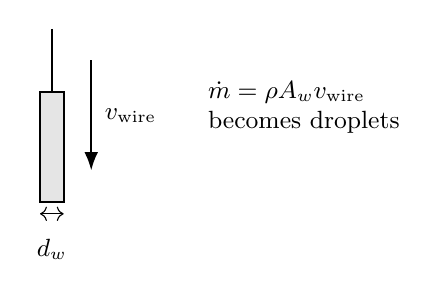
\begin{tikzpicture}[font=\small]
  \draw[thick] (0,1.2) -- (0,0.4);
  \draw[thick,fill=gray!20] (-0.15,0.4) rectangle (0.15,-1.0);
  \draw[-{Latex},thick] (0.5,0.8) -- (0.5,-0.6);
  \node[right] at (0.55,0.1) {$v_{\mathrm{wire}}$};
  \draw[<->] (-0.15,-1.15) -- (0.15,-1.15);
  \node[below] at (0,-1.35) {$d_w$};
  \node[align=left] at (3.2,0.2) {$\dot{m}=\rho A_w v_{\mathrm{wire}}$\\becomes droplets};
\end{tikzpicture}
\end{center}

\incode{Job fields: \code{process.wire_feed_m_min}, \code{process.wire_diameter_mm}.
Converted to SI in the twin; used by deposition / droplet sizing.}
\fref{\cite{Wang2003,Lancaster1986,waam_twin2025}}

\subsection{Droplet mass and volume}
\newbie{Metal does not arrive as a continuous hose of liquid in this model --- it
arrives as discrete droplets at frequency $f_{\mathrm{drop}}$. Each droplet carries
mass $\dot{m}/f_{\mathrm{drop}}$.}

\begin{align}
  m_{\mathrm{drop}} &= \dot{m}\,\Delta t_{\mathrm{drop}}
                    = \frac{\dot{m}}{f_{\mathrm{drop}}} \label{eq:mdrop}\\
  V_{\mathrm{drop}} &= \frac{m_{\mathrm{drop}}}{\rho} \label{eq:vdrop}
\end{align}
Equivalent spherical radius in grid cells (volume $V$, cell size $\Delta x$):
\begin{equation}
  r_{\mathrm{cells}} = \left(\frac{3V}{4\pi\,\Delta x^3}\right)^{1/3}
\end{equation}
\fref{\cite{Wang2003,Lancaster1986,waam_twin2025}}

\subsection{Travel speed and line energy}
\newbie{If the torch moves faster, the same watts are spread over more weld length,
so each millimetre of bead gets less energy. Line energy $q_{\mathrm{line}}$ captures that.}

\begin{equation}
  q_{\mathrm{line}} = \frac{Q_{\mathrm{eff}}}{v_{\mathrm{travel}}}
  \qquad [\mathrm{J/m}]
\end{equation}
\fref{\cite{Rosenthal1946,Goldak1984,Kou2003}}

%=============================================================================
\section{Governing conservation equations}
%=============================================================================

\subsection{Continuity}
\newbie{Mass is conserved: fluid cannot appear or disappear except where we
explicitly deposit wire. For nearly incompressible liquid metal, density is
almost constant $\rho_0$.}

\begin{equation}
  \frac{\partial \rho}{\partial t} + \nabla\cdot(\rho\vect{u}) = 0
\end{equation}
In the incompressible LBM liquid region, $\rho \approx \rho_0$.
\fref{\cite{Batchelor1967,Kruger2017}}

\subsection{Momentum (Navier--Stokes)}
\newbie{Newton's second law for a fluid: acceleration equals pressure forces +
viscous drag + gravity/body forces. All the weld-pool mechanisms (Marangoni,
Lorentz, arc pressure, \ldots) enter through $\vect{F}_{\mathrm{body}}$.}

\begin{equation}
  \rho\left(\frac{\partial \vect{u}}{\partial t} + \vect{u}\cdot\nabla\vect{u}\right)
  = -\nabla p + \nabla\cdot\bigl[\mu(\nabla\vect{u} + \nabla\vect{u}^{\mathsf T})\bigr]
  + \rho\vect{g} + \vect{F}_{\mathrm{body}}
  \label{eq:ns}
\end{equation}
\fref{\cite{Oreper1984,Kou2003,Incropera2007}}

\subsection{Energy / enthalpy}
\label{sec:energy}
\newbie{Instead of storing temperature alone, the twin stores volumetric enthalpy
$H$ [J/m$^3$]. That makes melting/freezing easier: latent heat is already inside
$H$. Heat moves by advection (carried with flow) and conduction; the arc adds
$\dot{q}_{\mathrm{arc}}$.}

\begin{equation}
  \frac{\partial H}{\partial t} + \vect{u}\cdot\nabla H = \nabla\cdot(k\nabla T) + \dot{q}_{\mathrm{arc}}
  \label{eq:enthalpy-transport}
\end{equation}
with $k = \rho c_p \alpha$ and $T$ recovered from $H$ (Section~\ref{sec:phase}).
\fref{\cite{Voller1987,Incropera2007,Brent1988}}

%=============================================================================
\section{Heat sources}
\label{sec:heat}
%=============================================================================

Valid job values today: \code{gaussian2d} or \code{goldak}
(aliases \code{goldak3d}, \code{doubleellipsoid}).
Set via \code{heat_source} in the job YAML. \code{conical} is \emph{not} implemented.

\subsection{Gaussian surface / near-surface source}
\newbie{Imagine a bell curve of heat under the torch: hottest at the centre,
weaker farther away. Radius $\sigma$ sets how wide the bell is.}

Analytic surface flux idea:
\begin{equation}
  q(r) = \frac{Q_{\mathrm{eff}}}{2\pi\sigma^2}\,
         \exp\!\left(-\frac{r^2}{2\sigma^2}\right)
  \label{eq:gaussian-flux}
\end{equation}

\textbf{What the twin actually does} (discrete, energy-safe): two passes over
metal cells --- (1)~sum Gaussian$\times$deposition weights $w$; (2)~deposit
\begin{equation}
  \Delta H_{ijk}
  = \frac{\eta\, Q_w\,\Delta t}{\bigl(\sum w\bigr)\,\Delta x^3}\, w_{ijk}
\end{equation}
so \emph{exactly} $\eta Q_w\Delta t$ joules enter metal every step, even if the
analytic footprint overhangs gas or the plate edge.

\begin{center}
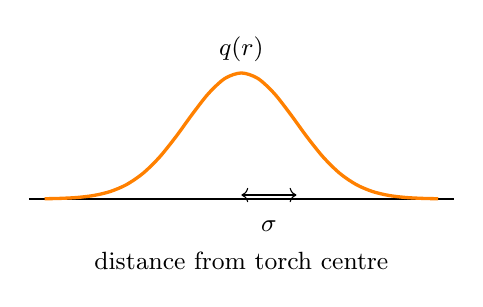
\begin{tikzpicture}[font=\small]
  \draw[thick] (-0.2,0) -- (5.2,0);
  \draw[domain=0:5,smooth,variable=\x,orange,very thick]
    plot ({\x},{1.6*exp(-((\x-2.5)^2)/(2*0.7^2))});
  \draw[<->] (2.5,0.05) -- (3.2,0.05);
  \node[below] at (2.85,-0.15) {$\sigma$};
  \node at (2.5,1.9) {$q(r)$};
  \node[below] at (2.5,-0.55) {distance from torch centre};
\end{tikzpicture}
\end{center}

\incode{\code{inject_arc_heat}; arc radius from \code{arc_physics.sigma_mm}
($\to$ \code{twin.sigma_cells}). Optional depth weighting via
\code{penetration_mm} / \code{arc_surface_weighting}.}
\fref{\cite{Rykalin1951,Goldak1984,waam_twin2025}}

\subsection{Goldak double-ellipsoid source}
\label{sec:goldak}
\newbie{Real arcs dump more heat behind the torch than in front (the pool trails
the motion). Goldak models this with two half-ellipsoids: a short, intense
\emph{front} and a longer \emph{rear}, with heat fractions $f_f$ and $f_r$.}

Classical Goldak (1984) power density (front or rear):
\begin{equation}
  q_{f,r}(\xi,y,z)
  = \frac{6\sqrt{3}\,f_{f,r}\,Q_{\mathrm{eff}}}{\pi\sqrt{\pi}\,a_{f,r}\,b\,c}
  \exp\!\left(
    -3\frac{\xi^2}{a_{f,r}^2}
    -3\frac{y^2}{b^2}
    -3\frac{z^2}{c^2}
  \right)
  \label{eq:goldak}
\end{equation}
with the Goldak convention
\begin{equation}
  f_f + f_r = 2
\end{equation}
(not $1$ --- the factor $2$ is part of the classical normalisation).
Semi-axes: $a$ along travel, $b$ transverse half-width, $c$ depth.

\begin{center}
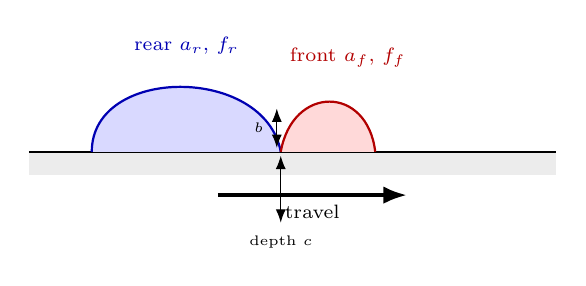
\begin{tikzpicture}[font=\scriptsize,>=Latex]
  % plate
  \fill[gray!15] (-3.2,-0.3) rectangle (3.5,0);
  \draw[thick] (-3.2,0) -- (3.5,0);
  % rear ellipsoid (longer)
  \draw[thick,blue!70!black,fill=blue!15]
    (-2.4,0) .. controls (-2.4,1.1) and (-0.2,1.1) .. (0,0);
  % front ellipsoid (shorter)
  \draw[thick,red!70!black,fill=red!15]
    (0,0) .. controls (0.15,0.85) and (1.1,0.85) .. (1.2,0);
  \draw[-{Latex},very thick] (-0.8,-0.55) -- (1.6,-0.55);
  \node[below] at (0.4,-0.55) {travel};
  \node[blue!70!black] at (-1.2,1.35) {rear $a_r$, $f_r$};
  \node[red!70!black] at (0.85,1.2) {front $a_f$, $f_f$};
  \draw[<->] (0,-0.05) -- (0,-0.9);
  \node[below] at (0,-0.95) {\tiny depth $c$};
  \draw[<->] (-0.05,0.05) -- (-0.05,0.55);
  \node[left] at (-0.1,0.3) {\tiny $b$};
\end{tikzpicture}
\end{center}

Typical defaults in jobs: $f_f=0.6$, $f_r=1.4$ (sum $=2$).
YAML axes (mm) map to cells via $\Delta x$:
\code{a_front_mm}, \code{a_rear_mm}, \code{b_mm}, \code{c_mm}.

\textbf{Implementation notes (current code):}
\begin{itemize}[leftmargin=*]
  \item Spatial weight follows the Goldak exponential
        $f\exp(-3\xi^2/a^2-3y^2/b^2-3z^2/c^2)$; the closed-form amplitude
        $6\sqrt{3}/(\pi\sqrt{\pi}abc)$ is absorbed by discrete energy
        renormalisation (same two-pass idea as Gaussian).
  \item Front/rear is chosen in the \emph{travel frame}:
        $\xi = (x-x_0)d_x + (y-y_0)d_y$ with unit torch direction
        $(d_x,d_y)$ from the path --- not fixed to grid $+x$.
  \item Loader enforces $f_f+f_r=2$ (\code{normalize_goldak_fractions}).
\end{itemize}

\incode{\path{physics/arc.py} (\code{Goldak3D}) and \code{inject_goldak_heat}.
See also \path{docs/PHYSICS_FORCE_CORRECTNESS_SPEC.md} §5.4.}
\fref{\cite{Goldak1984,Goldak1984b,waam_twin2025}}

\subsection{Arc deposition / penetration weight}
\newbie{Heat should land mostly near the free surface of the metal, not deep
inside solid plate. An optional exponential weight fades heat with depth below
the arc.}

\begin{equation}
  w_{\mathrm{dep}}(z) = \exp\!\left(-\frac{\max(0,\, z_{\mathrm{arc}}-z)}{\delta}\right)
\end{equation}
\incode{\code{arc_deposition_weight}; \code{arc_physics.penetration_mm},
\code{arc_surface_weighting} / \code{simulation.arc_surface_weighting}.}
\fref{\cite{Goldak1984,Rosenthal1946,waam_twin2025}}

\subsection{Rosenthal far-field check (validation only)}
\newbie{Rosenthal treats the arc as a moving point source. It is useful far from
the pool for cooling-rate checks, but \emph{not} used as the production heat
source in jobs.}

\begin{align}
  \sigma_R &= \frac{\rho c_p v}{2k} \\
  T - T_0 &= \frac{\eta Q}{2\pi k}\,\frac{1}{|x|}\,
            \exp(\sigma_R x), \qquad x < 0 \label{eq:rosenthal}
\end{align}
\incode{\code{validation/test_rosenthal_farfield.py}.}
\fref{\cite{Rosenthal1946,waam_twin2025}}

%=============================================================================
\section{Thermal transport and phase change}
\label{sec:phase}
%=============================================================================

\subsection{Fourier conduction}
\newbie{Heat flows from hot to cold, proportional to the temperature gradient.
Thermal diffusivity $\alpha=k/(\rho c_p)$ says how fast temperature spreads.}

\begin{equation}
  \vect{q} = -k\,\nabla T, \qquad
  \alpha = \frac{k}{\rho c_p}
\end{equation}
\fref{\cite{Incropera2007,Carslaw1959}}

\subsection{Enthalpy--porosity method}
\newbie{Solid, mushy, and liquid are encoded in $H$. Below solidus: all solid.
Between solidus and liquidus: mixture (liquid fraction $f_l$). Above liquidus:
all liquid, and extra enthalpy raises temperature further.}

Define
\begin{align}
  H_{\mathrm{sol}} &= \rho c_p\, T_s \\
  H_{\mathrm{liq}} &= H_{\mathrm{sol}} + \rho L_f
\end{align}

\begin{center}
\begin{tikzpicture}[font=\small,>=Latex]
  \draw[-{Latex}] (0,0) -- (6.2,0) node[right] {$H$};
  \draw[-{Latex}] (0,0) -- (0,3.2) node[above] {$T$};
  \draw[thick,blue!60!black] (0.3,0.4) -- (2.0,1.6) -- (3.6,2.2) -- (5.5,3.0);
  \draw[dashed] (2.0,0) -- (2.0,1.6);
  \draw[dashed] (3.6,0) -- (3.6,2.2);
  \node[below] at (2.0,-0.15) {$H_{\mathrm{sol}}$};
  \node[below] at (3.6,-0.15) {$H_{\mathrm{liq}}$};
  \node at (1.0,1.3) {\tiny solid};
  \node at (2.8,2.5) {\tiny mushy};
  \node at (4.7,2.0) {\tiny liquid};
  \node[left] at (0,1.6) {$T_s$};
  \node[left] at (0,2.2) {$T_l$};
\end{tikzpicture}
\end{center}

\textbf{Solid} ($H \le H_{\mathrm{sol}}$):
\begin{equation}
  f_l = 0, \qquad T = \frac{H}{\rho c_p}
\end{equation}
\textbf{Mushy} ($H_{\mathrm{sol}} < H < H_{\mathrm{liq}}$):
\begin{equation}
  f_l = \frac{H - H_{\mathrm{sol}}}{\rho L_f}, \qquad
  T = T_s + f_l\,(T_l - T_s)
\end{equation}
\textbf{Liquid} ($H \ge H_{\mathrm{liq}}$):
\begin{equation}
  f_l = 1, \qquad T = T_l + \frac{H - H_{\mathrm{liq}}}{\rho c_p}
\end{equation}
\incode{\code{kernels.update_phase} / thermal phase helpers.}
\fref{\cite{Voller1987,Brent1988,waam_twin2025}}

\subsection{Lattice thermal update}
In lattice units ($\alpha_{\mathrm{lu}} = \alpha\,\Delta t/\Delta x^2$):
\begin{equation}
  \frac{\partial H}{\partial t}\Big|_{\mathrm{cell}}
  = -\vect{u}\cdot\nabla H + \rho c_p\,\alpha_{\mathrm{lu}}\,\nabla^2 T
\end{equation}
(first-order upwind advection, central diffusion; variable-$c_p$ path when
material tables are on).
\fref{\cite{Incropera2007,Patankar1980,waam_twin2025}}

\subsection{Enthalpy ceiling (vaporization cap)}
\newbie{Without a cap, a tiny cell under the arc can spike to absurd temperatures.
A vapor enthalpy ceiling clips $H$ near boiling / vaporisation.}

\begin{equation}
  H \le H_{\mathrm{vap}} \approx \rho c_p\, T_{\mathrm{vap,cap}} + \rho L_{\mathrm{vap}}
\end{equation}
(gated by \code{enable_enthalpy_cap}, temperature from \code{T_vapor_cap_K}).
\fref{\cite{Matsunawa1997,waam_twin2025}}

\subsection{Evaporative cooling (surface sink)}
\newbie{When the surface approaches boiling, evaporation removes enthalpy
(energy leaves with vapour). This is separate from the hard ceiling and from
recoil pressure.}

Phenomenological sink on interface cells for $T$ above an onset toward $T_b$,
scaled by job key \code{evap_cooling_scale} (under \code{advanced_physics}) and $L_v$.
\incode{\code{apply_evaporative_enthalpy_sink}; flag \code{enable_evaporative_cooling}.
Onset shared with Clausius--Clapeyron recoil.}
\fref{\cite{Matsunawa1997,Semak1997,waam_twin2025}}

\subsection{Stefan solidification benchmark}
\begin{align}
  \mathrm{Ste} &= \frac{c_p\,(T_{\mathrm{init}} - T_0)}{L_f} \\
  \sqrt{\pi}\,\lambda\,\exp(\lambda^2)\,\mathrm{erf}(\lambda) &= \mathrm{Ste} \\
  s(t) &= 2\lambda\sqrt{\alpha t}
\end{align}
\incode{\code{validation/test_stefan_solidification.py}.}
\fref{\cite{Carslaw1959,Crank1984,waam_twin2025}}

\subsection{Boundary heat losses}
\newbie{The bead and plate lose heat to air by convection and radiation.}

On gas-exposed faces:
\begin{align}
  q_{\mathrm{loss}} &= h_{\mathrm{conv}}\,(T - T_{\mathrm{amb}})
                    + \varepsilon\,\sigma_{\mathrm{SB}}\,(T^4 - T_{\mathrm{amb}}^4) \\
  H &\leftarrow H - q_{\mathrm{loss}}\,\frac{\Delta t}{\Delta x}
\end{align}
($H$ is volumetric; dividing by $\Delta x$ converts a surface flux to a cell update.)
\incode{\code{enable_heat_loss}, \code{heat_loss.h_conv}, radiation flag.}
\fref{\cite{Incropera2007,Kou2003,waam_twin2025}}

%=============================================================================
\section{Lattice Boltzmann numerics}
%=============================================================================

\subsection{Lattice units}
\newbie{Physical metres and seconds are converted to dimensionless lattice units
so the LBM stays stable (small Mach number).}

\begin{align}
  \Delta t &= \Delta x\,\frac{u_{\mathrm{ref,lu}}}{u_{\mathrm{ref,phys}}} \\
  \nu_{\mathrm{lu}} &= \frac{\mu}{\rho}\,\frac{\Delta t}{\Delta x^2}, \qquad
  \tau = 3\nu_{\mathrm{lu}} + \tfrac{1}{2} \\
  \alpha_{\mathrm{lu}} &= \alpha\,\frac{\Delta t}{\Delta x^2}, \qquad
  \tau_T = 3\alpha_{\mathrm{lu}} + \tfrac{1}{2}
\end{align}
Target Mach $\mathrm{Ma} \approx u_{\mathrm{ref,phys}}\,\Delta t/\Delta x \sim 0.05$.
\fref{\cite{Kruger2017,Chen1998,waam_twin2025}}

\subsection{D3Q19 equilibrium (SRT)}
\begin{equation}
  f_i^{\mathrm{eq}} = w_i\,\rho
  \left(1 + 3\,\vect{e}_i\cdot\vect{u}
  + \tfrac{9}{2}(\vect{e}_i\cdot\vect{u})^2
  - \tfrac{3}{2}\vect{u}^2\right)
\end{equation}
\fref{\cite{Qian1992,Kruger2017,Chen1998}}

\subsection{Guo forcing scheme (2002)}
\newbie{Body forces (Marangoni, gravity, \ldots) are added inside LBM collision
using Guo's method so the Navier--Stokes force term is recovered.}

\begin{align}
  \vect{u}^\ast &= \vect{u} + \frac{\tau}{\rho}\,\vect{F} \\
  S_i &= w_i\left(1 - \frac{\omega}{2}\right)
  \left[3\,\vect{e}_i\cdot\vect{F}
  + 9(\vect{e}_i\cdot\vect{u})(\vect{e}_i\cdot\vect{F})
  - 3\,\vect{u}\cdot\vect{F}\right]
\end{align}
Lattice force scaling (physical force density $\vect{f}_{\mathrm{phys}}$):
\begin{equation}
  \vect{a}_{\mathrm{lu}}
  = \frac{\vect{f}_{\mathrm{phys}}}{\rho}\,\frac{\Delta t^2}{\Delta x}
\end{equation}
\fref{\cite{Guo2002,Kruger2017,waam_twin2025}}

\subsection{Carman--Kozeny mushy-zone drag}
\newbie{In the mushy zone, solid dendrites act like a porous sponge. Velocity is
dragged toward zero as $f_l\to 0$.}

\begin{equation}
  \vect{u}_{\mathrm{final}} = \frac{\vect{u}^\ast}
  {1 + C_K\,\dfrac{(1-f_l)^2}{f_l^3 + \varepsilon}}
\end{equation}
\fref{\cite{Voller1987,Poirier1987,waam_twin2025}}

%=============================================================================
\section{Free surface (VOF) and surface tension}
%=============================================================================

\subsection{VOF phase field}
\newbie{$\phi=1$ means ``full of metal'', $\phi=0$ means gas. The free surface
is where $\phi$ transitions. Tracking $\phi$ lets the bead crown move.}

Volume fraction $\phi \in [0,1]$; interface where $|\nabla\phi| > \varepsilon$.
\fref{\cite{Hirt1981,Rider2001}}

\subsection{Continuum Surface Force (CSF)}
\newbie{Surface tension pulls the interface toward lower curvature (wants a
smoother, rounder surface). CSF turns that into a volumetric force near the interface.}

\begin{align}
  \unit{n} &= \frac{\nabla\phi}{|\nabla\phi|} \\
  \kappa &= -\nabla\cdot\unit{n} \\
  \vect{F}_{\mathrm{CSF}} &= \gamma\,\kappa\,\nabla\phi
\end{align}
\fref{\cite{Brackbill1992,waam_twin2025}}

\subsection{Marangoni force}
\newbie{Surface tension depends on temperature. For many pure metals
$\mathrm{d}\gamma/\mathrm{d}T < 0$: hotter surface has weaker tension, so liquid
is pulled toward cooler edges --- outward surface flow.}

\begin{align}
  \nabla_s T &= (\mathbf{I} - \unit{n}\unit{n}^{\mathsf T})\,\nabla T \\
  \vect{F}_M &= \frac{\mathrm{d}\gamma}{\mathrm{d}T}\,\nabla_s T\,|\nabla\phi|
  \label{eq:marangoni}
\end{align}

\begin{center}
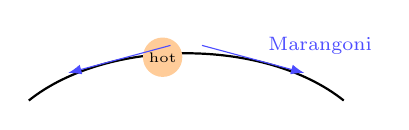
\begin{tikzpicture}[font=\scriptsize,>=Latex]
  \draw[thick] (-2,0) .. controls (-1,0.8) and (1,0.8) .. (2,0);
  \fill[orange!40] (-0.3,0.55) circle (0.25);
  \node at (-0.3,0.55) {\tiny hot};
  \draw[-{Latex},blue!70] (0.2,0.7) -- (1.5,0.35);
  \draw[-{Latex},blue!70] (-0.2,0.7) -- (-1.5,0.35);
  \node[blue!70] at (1.7,0.7) {Marangoni};
\end{tikzpicture}
\end{center}

Surfactants (S, O) can flip $\mathrm{d}\gamma/\mathrm{d}T$ and reverse circulation.
\fref{\cite{Kou2003,Davis1987,Oreper1984,waam_twin2025}}

\subsection{Wetting and contact angle}
Young's law:
\begin{equation}
  \cos\theta = \frac{\gamma_{sv} - \gamma_{sl}}{\gamma_{lv}}
\end{equation}
Effective interface normal at wall (Ding--Spelt style):
\begin{equation}
  \unit{n}_{\mathrm{eff}} = \sin\theta\,\unit{n}_{\mathrm{wall}}
  + \cos\theta\,\unit{t}_{\mathrm{wall}}
\end{equation}
Capillary length $\lambda_c = \sqrt{\gamma/(\rho g)}$; Bond number
$\mathrm{Bo}=\rho g L^2/\gamma$.
\incode{\code{enable_wetting}, \code{surface_wetting.contact_angle_deg}.}
\fref{\cite{deGennes2004,Brackbill1992,Ding2008,BEAD2025,waam_twin2025}}

%=============================================================================
\section{Weld-pool body and surface forces}
\label{sec:forces}
%=============================================================================

\newbie{After heat melts metal, \emph{forces} shape the pool: surface tension,
temperature-driven shear, electromagnetic pinch, gas jet, vapour recoil, gravity.
They are cleared once per step, then added with \texttt{+=} (never overwriting).}

Target force density:
\begin{equation}
\begin{aligned}
\mathbf{F}_{\mathrm{total}}
&=
\gamma\kappa\nabla\phi
+ \frac{\mathrm{d}\gamma}{\mathrm{d}T}\,\nabla_s T\,|\nabla\phi|
+ \unit{n}\,p_{\mathrm{arc}}
+ \unit{n}\,p_{\mathrm{recoil}}
+ \boldsymbol{\tau}_{\mathrm{gas}}
+ \unit{n}\,p_{\mathrm{drop}} \\
&\quad
+ \vect{J}\times\vect{B}
+ \rho\vect{g}\,f_l
- \rho g\beta(T-T_{\mathrm{ref}})\,\hat{\vect{z}}\,f_l
\end{aligned}
\end{equation}
(Sign of Boussinesq: $+z$ upward $\Rightarrow$ hot fluid rises; code uses
consistent lattice $g$.)

\subsection{Lorentz (electromagnetic) force}
\begin{equation}
  \vect{F}_{\mathrm{em}} = \vect{J}\times\vect{B}
  \label{eq:lorentz}
\end{equation}
Potential / Ohm / magnetostatic assembly in conductive metal; gated by
\code{enable_lorentz}.
\fref{\cite{Oreper1984,Jackson1986,waam_twin2025}}

\subsection{Boussinesq buoyancy and hydrostatic gravity}
\begin{align}
  F_z^{\mathrm{Buoy}} &= -\rho\,g\,\beta\,(T - T_{\mathrm{ref}})\,f_l
  \label{eq:boussinesq}\\
  \vect{F}_g &= \rho\,\vect{g}\,f_l, \qquad
  \vect{g} = (0,\,0,\,-g)
  \label{eq:hydrostatic}
\end{align}
\incode{\code{enable_buoyancy}, \code{enable_hydrostatic_gravity}.}
\fref{\cite{Oreper1984,Kou2003,waam_twin2025,BEAD2025}}

\subsection{Arc pressure (Lin--Eagar)}
\newbie{The arc also pushes down on the pool surface (like a soft jet). Peak
pressure scales with $I^2$.}

Default model (\code{arc_physics.pressure_model: lin_eagar}):
\begin{equation}
  p_0(I)=\frac{\mu_0 I^2}{4\pi^2 \sigma_p^2}, \qquad
  p_{\mathrm{arc}}(r)=p_0\exp\!\left(-\frac{r^2}{2\sigma_p^2}\right)
\end{equation}
Alternative: constant \code{pressure_pa}.
\incode{\code{physics/weld_forces.py} \code{lin_eagar_peak_pa}.}
\fref{\cite{Oreper1984,Tanaka2006,waam_twin2025}}

\subsection{Vapor recoil}
\textbf{Clausius--Clapeyron} (preferred when enabled):
\begin{equation}
  P_{\mathrm{vap}}(T) = C_{\mathrm{acc}}\,P_{\mathrm{ref}}\,
  \exp\!\left[\frac{L_v}{R_v}
  \left(\frac{1}{T_b} - \frac{1}{T}\right)\right]
  \quad (T \gtrsim T_{\mathrm{onset}})
\end{equation}
\incode{\code{enable_recoil}, \code{use_recoil_clausius_clapeyron},
\code{recoil_accommodation}. Often off for conduction-mode WAAM.}
\fref{\cite{Matsunawa1997,Semak1997,waam_twin2025}}

\subsection{Gas-jet shear}
\begin{equation}
  \tau_{\mathrm{gas}} = \tfrac{1}{2}\,\rho_{\mathrm{gas}}\,v_{\mathrm{jet}}^2\,C_{\tau}
\end{equation}
\incode{\code{enable_gas_shear}, \code{gas_jet_velocity_m_s}.}
\fref{\cite{Mills2010,Oreper1984,waam_twin2025}}

%=============================================================================
\section{Droplet deposition and impact}
\label{sec:droplet}
%=============================================================================

\subsection{Mass balance}
\begin{equation}
  m_{\mathrm{dep,expected}} = \dot{m}\,t, \qquad
  \chi_m = \frac{m_{\mathrm{dep,sim}}}{m_{\mathrm{dep,expected}}} \approx 1
\end{equation}
\fref{\cite{waam_twin2025,Wang2003}}

\subsection{Impact velocity and pressure}
\begin{align}
  L_{\mathrm{drop}} &\approx \frac{v_{\mathrm{wire}}}{f_{\mathrm{drop}}} \\
  v_{\mathrm{grav}} &= \sqrt{2g L_{\mathrm{drop}}} \\
  v_{\mathrm{impact}} &\approx f_{\mathrm{mode}}\,
  \max\!\left(v_{\mathrm{wire}},\, v_{\mathrm{grav}} + v_{\mathrm{pinch}}\right)
\end{align}
\begin{equation}
  p_{\mathrm{impact}} \approx
  \frac{\tfrac{1}{2}\,m_{\mathrm{drop}}\,v_{\mathrm{impact}}^2}{\pi r_{\mathrm{contact}}^2}
\end{equation}
Droplet enthalpy:
\begin{equation}
  H_{\mathrm{drop}} = \rho c_p\, T_{\mathrm{drop}} + \rho L_f, \qquad
  T_{\mathrm{drop}} = T_l + \Delta T_{\mathrm{superheat}}
\end{equation}
(+ stick-out preheat when enabled).
\fref{\cite{Wang2003,Lancaster1986,Bernhardi2005,waam_twin2025}}

%=============================================================================
\section{Electrical stick-out and CTWD}
%=============================================================================

\begin{align}
  R_{\mathrm{stick}} &= \frac{\rho_e\,L_{\mathrm{stick}}}{A_w} \\
  P_{\mathrm{preheat}} &= \eta_{\mathrm{stick}}\,I^2 R_{\mathrm{stick}} \\
  \Delta T_{\mathrm{preheat}} &= \frac{P_{\mathrm{preheat}}}{\dot{m}\,c_p}
\end{align}
CTWD drift with measured bead height:
\begin{equation}
  \mathrm{CTWD}_{n+1} = \mathrm{CTWD}_{\mathrm{nominal}}
  + \left(h_{\mathrm{bead,measured}} - h_{\mathrm{layer,planned}}\right)
\end{equation}
\fref{\cite{Klaus2022,Incropera2007,BEAD2025,waam_twin2025}}

%=============================================================================
\section{Material properties}
%=============================================================================

\begin{align}
  c_{p,\rho} &= \rho\,c_p \quad [\mathrm{J/(m^3\,K)}] \\
  L_\rho &= \rho\,L_f \quad [\mathrm{J/m^3}] \\
  \gamma(T) &\approx \gamma_0 + \frac{\mathrm{d}\gamma}{\mathrm{d}T}\,(T - T_{\mathrm{ref}})
\end{align}
Optional piecewise-linear tables in material YAML for $\mu(T)$, $k(T)$, $c_p(T)$.
\fref{\cite{Incropera2007,Kou2003,waam_twin2025}}

%=============================================================================
\section{Bead geometry metrics}
%=============================================================================

\begin{center}
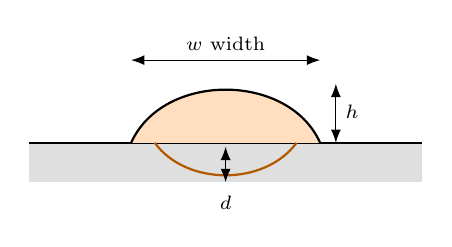
\begin{tikzpicture}[font=\scriptsize,>=Latex]
  \fill[gray!25] (-2.5,0) rectangle (2.5,-0.5);
  \draw[thick] (-2.5,0) -- (2.5,0);
  \draw[thick,fill=orange!25]
    (-1.2,0) .. controls (-0.8,0.9) and (0.8,0.9) .. (1.2,0);
  \draw[thick,orange!70!black]
    (-0.9,0) .. controls (-0.5,-0.55) and (0.5,-0.55) .. (0.9,0);
  \draw[<->] (-1.2,1.05) -- (1.2,1.05);
  \node[above] at (0,1.05) {$w$ width};
  \draw[<->] (1.4,0) -- (1.4,0.75);
  \node[right] at (1.4,0.4) {$h$};
  \draw[<->] (0,-0.05) -- (0,-0.5);
  \node[below] at (0,-0.55) {$d$};
\end{tikzpicture}
\end{center}

\begin{align}
  w_{\mathrm{pool}} &= \text{transverse liquid extent at surface} \\
  d_{\mathrm{pool}} &= \text{penetration below substrate} \\
  h_{\mathrm{bead}} &= \text{deposit height above substrate} \\
  \theta_{\mathrm{toe}} &\approx \text{contact angle at triple line}
\end{align}
\fref{\cite{waam_twin2025,Kou2003,BEAD2025}}

%=============================================================================
\section{Coordinate frames (robot integration)}
%=============================================================================

KUKA TCP [mm] $\to$ simulation metres:
\begin{align}
  x_{\mathrm{sim}} &= \frac{x_{\mathrm{TCP,mm}} - x_{\mathrm{origin,mm}}}{1000} - x_{\mathrm{offset,m}} \\
  y_{\mathrm{sim}} &= \frac{y_{\mathrm{TCP,mm}} - y_{\mathrm{origin,mm}}}{1000} - y_{\mathrm{offset,m}} \\
  z_{\mathrm{sim}} &= \frac{z_{\mathrm{TCP,mm}} - z_{\mathrm{origin,mm}}}{1000}
\end{align}
Torch $z$ vs CTWD conventions are handled in \code{coupled_step._resolve_arc_k}.
\fref{\cite{waam_twin2025,KUKA2024}}

%=============================================================================
\section{Digital twin platform signals}
%=============================================================================

\begin{equation}
  \mathcal{U}(t) = \bigl\{t,\, x,\, y,\, z,\, I,\, V,\, \mathrm{WFS},\, \mathrm{is\_welding},\, \mathrm{material\_id}\bigr\}
\end{equation}
\begin{equation}
  \mathcal{S}(t+\Delta t) = \mathrm{WAAMTwin.step}\bigl(\mathcal{U}(t)\bigr)
\end{equation}
Supervisory deviation: $\Delta y = y_{\mathrm{meas}} - y_{\mathrm{twin}}$.
\fref{\cite{ARCH2025,ISO23247,Grieves2014,Klaus2022,Astrom2008}}

%=============================================================================
\section{Physics tiers (current project)}
\label{sec:tiers}
%=============================================================================

\newbie{Not every run needs every force. Jobs select a \emph{physics tier} so
you can debug thermal behaviour alone, or turn on full weld-pool mechanics.}

\begin{center}
\small
\begin{tabular}{@{}p{2.4cm}p{3.2cm}p{8.2cm}@{}}
\toprule
Tier & Intent & Typical enables \\
\midrule
\code{thermal} & heat + phase only & no VOF / CSF / Marangoni / MHD \\
\code{flow} & free-surface flow & + VOF, CSF, Marangoni, buoyancy, gravity, droplets \\
\code{full} & production catalogue & + Lorentz, Lin--Eagar arc pressure, gas shear, wetting, \ldots \\
\bottomrule
\end{tabular}
\end{center}
Set the tier with \code{simulation.physics_tier} in the job YAML.

Recoil remains an explicit flag (\code{enable_recoil}); conduction-mode WAAM often
leaves it off. Example: \code{jobs/examples/bead_on_plate_hires.yaml} uses
\code{physics_tier: full} with Goldak + many force flags on.

%=============================================================================
\section{Dimensionless groups}
%=============================================================================

\begin{align}
  \mathrm{Re} &= \frac{\rho U L}{\mu} &
  \mathrm{Pr} &= \frac{\nu}{\alpha} \\
  \mathrm{Pe} &= \frac{U L}{\alpha} &
  \mathrm{Ma}_{\mathrm{LBM}} &\approx \frac{u_{\mathrm{ref}}\,\Delta t}{\Delta x} \\
  \mathrm{We} &= \frac{\rho U^2 L}{\gamma} &
  \mathrm{Bo} &= \frac{\rho g L^2}{\gamma}
\end{align}
\fref{\cite{Batchelor1967,Incropera2007,Kruger2017}}

%=============================================================================
\section{Coupled timestep order (current code)}
\label{sec:step}
%=============================================================================

Per-step sequence in \code{solvers/coupled_step.py} (simplified):

\begin{enumerate}[leftmargin=*]
  \item Resolve arc location on the free surface / torch $z$.
  \item Arc heat injection (Gaussian or Goldak) $\rightarrow$ wire droplets
        $\rightarrow$ droplet impact pressure/momentum.
  \item Thermal advection--diffusion; boundary losses; phase update.
  \item Evaporative cooling (optional); enthalpy vapor cap.
  \item Optional bead freeze / substrate growth solidification.
  \item VOF advection, reinit, wetting BC, flag update.
  \item \textbf{clear forces}, then add: CSF (+wetting) $\rightarrow$ Marangoni
        $\rightarrow$ gas shear $\rightarrow$ arc pressure $\rightarrow$ recoil
        $\rightarrow$ hydrostatic gravity $\rightarrow$ Boussinesq $\rightarrow$ Lorentz.
  \item Force/Mach clamps (stability); LBM collide (Darcy in mush) $\rightarrow$ stream.
  \item Tracer advection; thermal-history accumulators; force snapshot.
\end{enumerate}

\begin{center}
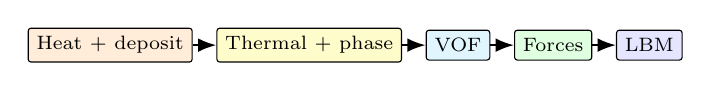
\begin{tikzpicture}[
  font=\scriptsize,
  box/.style={draw,rounded corners=1pt,align=center,inner sep=3pt},
  arr/.style={-{Latex},thick}
]
\node[box,fill=orange!15] (a) {Heat + deposit};
\node[box,fill=yellow!20,right=3mm of a] (b) {Thermal + phase};
\node[box,fill=cyan!12,right=3mm of b] (c) {VOF};
\node[box,fill=green!12,right=3mm of c] (d) {Forces};
\node[box,fill=blue!10,right=3mm of d] (e) {LBM};
\draw[arr] (a) -- (b);
\draw[arr] (b) -- (c);
\draw[arr] (c) -- (d);
\draw[arr] (d) -- (e);
\end{tikzpicture}
\end{center}

\fref{\cite{waam_twin2025,Voller1987,Brackbill1992,Guo2002}}

%=============================================================================
\section{Quick symbol sheet}
%=============================================================================

\begin{center}
\begin{tabular}{@{}lll@{}}
\toprule
Symbol & Meaning & SI \\
\midrule
$I,V$ & arc current, voltage & A, V \\
$\eta$ & arc thermal efficiency & -- \\
$Q_w$ & electrical power in code ($IV$) & W \\
$Q_{\mathrm{eff}}$ & $\eta IV$ useful heat rate & W \\
$\dot{q}_{\mathrm{arc}}$ & local arc heat density & W/m$^3$ \\
$H$ & volumetric enthalpy & J/m$^3$ \\
$f_l$ & liquid fraction & -- \\
$\phi$ & VOF metal fraction & -- \\
$a_f,a_r,b,c$ & Goldak semi-axes & m (mm in YAML) \\
$f_f,f_r$ & Goldak heat fractions ($f_f+f_r=2$) & -- \\
\bottomrule
\end{tabular}
\end{center}

%=============================================================================
\section{Bibliography}
%=============================================================================

\begin{thebibliography}{99}

\bibitem{ARCH2025}
WAAM Digital Twin Architecture (2025).
\textit{WAAM\_DIGITAL\_TWIN\_ARCHITECTURE.md}, FYP22-01/waam\_twin project.

\bibitem{BEAD2025}
Bead Geometry Physics Spec (2025).
\textit{BEAD\_GEOMETRY\_PHYSICS\_SPEC.md}, FYP22-01/waam\_twin project.

\bibitem{waam_twin2025}
\texttt{waam\_twin} GPU melt-pool digital twin (2024--2026).
Modules: \texttt{kernels/}, \texttt{physics/}, \texttt{solvers/coupled\_step.py},
\texttt{docs/PHYSICS\_FORCE\_CORRECTNESS\_SPEC.md}.

\bibitem{Astrom2008}
{\AA}str\"om, K.~J., and Murray, R.~M. (2008).
\textit{Feedback Systems}. Princeton University Press.

\bibitem{Batchelor1967}
Batchelor, G.~K. (1967).
\textit{An Introduction to Fluid Dynamics}. Cambridge University Press.

\bibitem{Bernhardi2005}
Bernhardi, L., and Duffie, N.~A. (2005).
Heat transfer and geometry model for gas metal arc welding.
\textit{Science and Technology of Welding and Joining}, 10(5), 581--587.

\bibitem{Brent1988}
Brent, A.~D., Voller, V.~R., and Reid, K.~J. (1988).
Enthalpy--porosity technique for modeling convection-diffusion phase change.
\textit{Numerical Heat Transfer}, 13(3), 297--318.

\bibitem{Brackbill1992}
Brackbill, J.~U., Kothe, D.~B., and Zemach, C. (1992).
A continuum method for modeling surface tension.
\textit{Journal of Computational Physics}, 100(2), 335--354.

\bibitem{Carslaw1959}
Carslaw, H.~S., and Jaeger, J.~C. (1959).
\textit{Conduction of Heat in Solids} (2nd ed.). Oxford University Press.

\bibitem{Chen1998}
Chen, S., and Doolen, G.~D. (1998).
Lattice Boltzmann method for fluid flows.
\textit{Annual Review of Fluid Mechanics}, 30, 329--364.

\bibitem{Crank1984}
Crank, J. (1984).
\textit{Free and Moving Boundary Problems}. Oxford University Press.

\bibitem{Davis1987}
Davis, S.~H. (1987).
Thermocapillary flows.
\textit{Annual Review of Fluid Mechanics}, 19, 403--435.

\bibitem{deGennes2004}
de~Gennes, P.-G., Brochard-Wyart, F., and Qu\'er\'e, D. (2004).
\textit{Capillarity and Wetting Phenomena}. Springer.

\bibitem{Ding2008}
Ding, H., and Spelt, P.~D.~M. (2008).
Wetting condition in multiphase lattice Boltzmann simulations.
\textit{Journal of Computational Physics}, 227(11), 5671--5690.

\bibitem{Goldak1984}
Goldak, J.~A., Chakravarti, A., and Bibby, M. (1984).
A new finite element model for computing heat flow in welds.
\textit{Welding Journal}, 63(10), 299s--305s.

\bibitem{Goldak1984b}
Goldak, J.~A., and Akhlaghi, M. (1984).
Computational weld pool geometry.
\textit{Welding Journal}, 63(10), 306s--312s.

\bibitem{Grieves2014}
Grieves, M., and Vickers, J. (2017).
Digital twin: Mitigating unpredictable, undesirable emergent behavior in complex systems.
In \textit{Transdisciplinary Perspectives on Complex Systems}. Springer.

\bibitem{Guo2002}
Guo, Z., Zheng, C., and Shi, B. (2002).
Discrete lattice effects on the forcing term in the lattice Boltzmann method.
\textit{Physical Review E}, 65(4), 046308.

\bibitem{Hirt1981}
Hirt, C.~W., and Nichols, B.~D. (1981).
Volume of fluid (VOF) method for the dynamics of free boundaries.
\textit{Journal of Computational Physics}, 39(1), 201--225.

\bibitem{Incropera2007}
Incropera, F.~P., et al. (2007).
\textit{Fundamentals of Heat and Mass Transfer} (6th ed.). Wiley.

\bibitem{ISO23247}
ISO (2021).
\textit{ISO 23247-1: Digital twin framework for manufacturing}.

\bibitem{Jackson1986}
Jackson, J.~D. (1999).
\textit{Classical Electrodynamics} (3rd ed.). Wiley.

\bibitem{Klaus2022}
Klaus, A., et al. (2022).
Short-circuit resistance and CTWD effects in GMAW
(basis cited in \textit{BEAD\_GEOMETRY\_PHYSICS\_SPEC.md}).

\bibitem{Kou2003}
Kou, S. (2003).
\textit{Welding Metallurgy} (2nd ed.). John Wiley \& Sons.

\bibitem{Kruger2017}
Kr\"uger, T., et al. (2017).
\textit{The Lattice Boltzmann Method: Principles and Practice}. Springer.

\bibitem{KUKA2024}
KUKA robot integration bridge (2024--2026).
\texttt{kuka\_adapter.py}, \texttt{frame.py}.

\bibitem{Lancaster1986}
Lancaster, J.~F. (1986).
\textit{The Physics of Welding} (2nd ed.). Pergamon Press.

\bibitem{Matsunawa1997}
Matsunawa, A., and Semak, V. (1997).
The simulation of front keyhole wall dynamics during laser welding.
\textit{Journal of Physics D}, 30(5), 798--809.

\bibitem{Mills2010}
Mills, K.~C., et al. (1998).
Marangoni effects in welding.
\textit{Phil.\ Trans.\ R.\ Soc.\ A}, 356, 911--935.

\bibitem{Oreper1984}
Oreper, G.~M., and Szekely, J. (1984).
Heat and fluid flow phenomena in weld pools.
\textit{Journal of Fluid Mechanics}, 147, 53--79.

\bibitem{Patankar1980}
Patankar, S.~V. (1980).
\textit{Numerical Heat Transfer and Fluid Flow}. Hemisphere.

\bibitem{Poirier1987}
Poirier, G.~E. (1987).
Permeability for flow parallel to a fiber axis.
\textit{Metallurgical Transactions B}, 18, 245--255.

\bibitem{Qian1992}
Qian, Y.~H., d'Humi\`eres, D., and Lallemand, P. (1992).
Lattice BGK models for Navier--Stokes equation.
\textit{Europhysics Letters}, 17, 479--484.

\bibitem{Radaj2003}
Radaj, D. (2003).
\textit{Welding Residual Stresses and Distortion}. Woodhead.

\bibitem{Rider2001}
Rider, W.~J., and Kothe, D.~B. (1998).
Reconstructing volume tracking.
\textit{Journal of Computational Physics}, 141, 112--152.

\bibitem{Rosenthal1946}
Rosenthal, D. (1946).
The theory of moving sources of heat and its application to metal treatments.
\textit{Transactions of the ASME}, 68, 849--866.

\bibitem{Rykalin1951}
Rykalin, N.~N. (1951).
\textit{Berechnung der W\"armevorg\"ange beim Schwei{\ss}en}. Akademie-Verlag.

\bibitem{Semak1997}
Semak, V.~V., and Matsunawa, A. (1997).
The role of recoil pressure in energy balance during laser materials processing.
\textit{Journal of Physics D}, 30(18), 2541--2552.

\bibitem{Tanaka2006}
Tanaka, M., and Lowke, J.~J. (2007).
Predictions of properties of free burning arcs.
\textit{Plasma Sources Sci.\ Technol.}, 16, 1--12.

\bibitem{Voller1987}
Voller, V.~R., and Prakash, C. (1987).
A fixed grid numerical modelling methodology for convection-diffusion mushy region phase-change problems.
\textit{Int.\ J.\ Heat Mass Transfer}, 30, 1709--1719.

\bibitem{Wang2003}
Wang, G., Hu, S.~J., and Carlson, B.~E. (2003).
Modelling and analysis of metal transfer in gas metal arc welding.
\textit{Journal of Physics D}, 36, 1143--1152.

\end{thebibliography}

\end{document}
